
This appendix compares the kinematic distributions for the truth objects in events that pass both the
the reconstruction level and truth let event selection to those that pass the truth selection 
but fail the reconstruction event selection.   Failed events are divided into categories based on which object fails
the reconstruction selection.  The selection cuts are applied in the order given in the figure legends.  Events that
fail one cut are not tested against subsequent cuts.  A subset of the figures from this section are also presented
in Figure~\ref{fig:truthnotreco}.

The true $b$-jet \pt\ and $\eta$  are shown in Figure~\ref{fig:norecobjet}.
The \pt\ distribution for extra truth jets of rank 1 through 5 are provided in Figure~\ref{fig:norecojetpt}. 
Figure~\ref{fig:norecojetmult} presents the true extra jet
jet multiplicity for different values of the jet \pt\ cut.

\begin{figure}[bth]
\centering
\begin{subfigure}[]{0.45\textwidth}
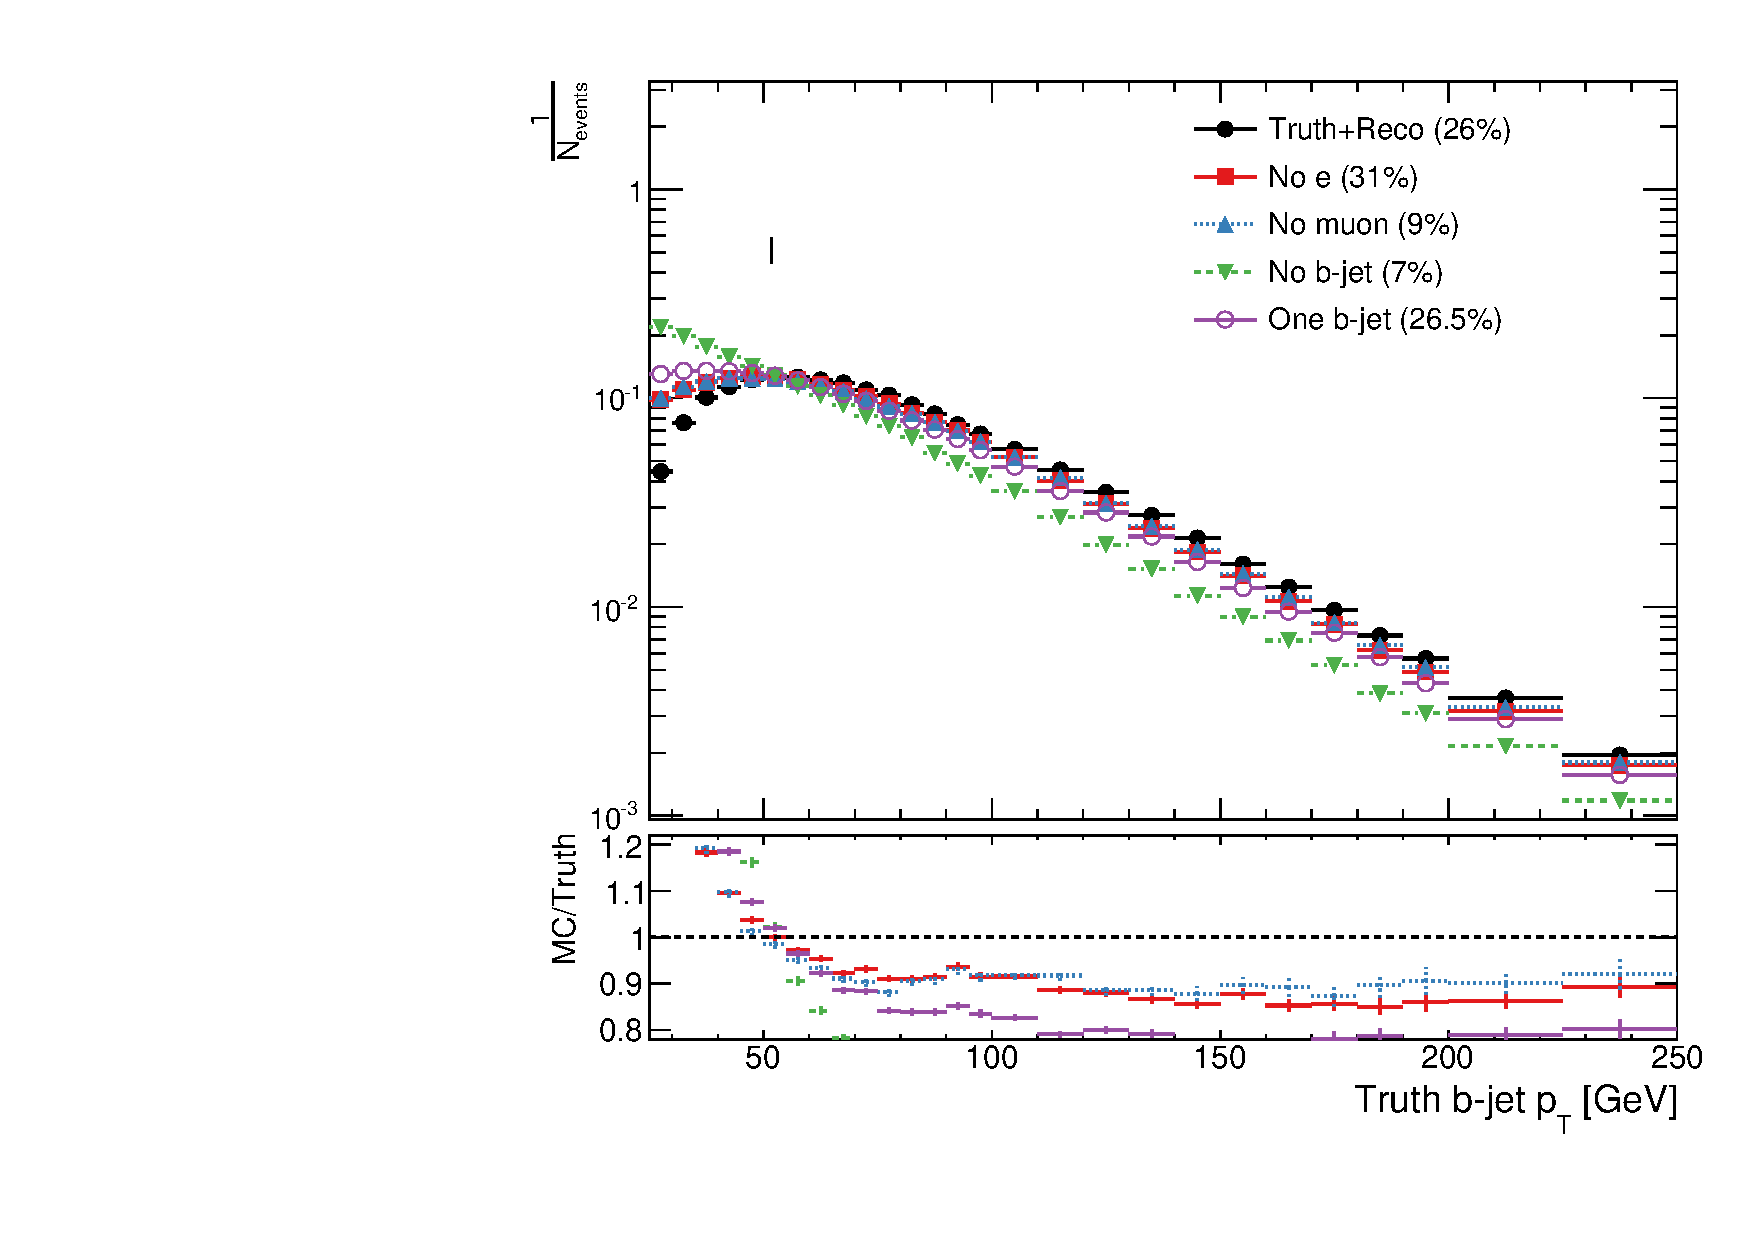
\includegraphics[width=\textwidth]{fig/TruthNotReco/TruthBJetPt.pdf}
\end{subfigure}
\begin{subfigure}[]{0.45\textwidth}
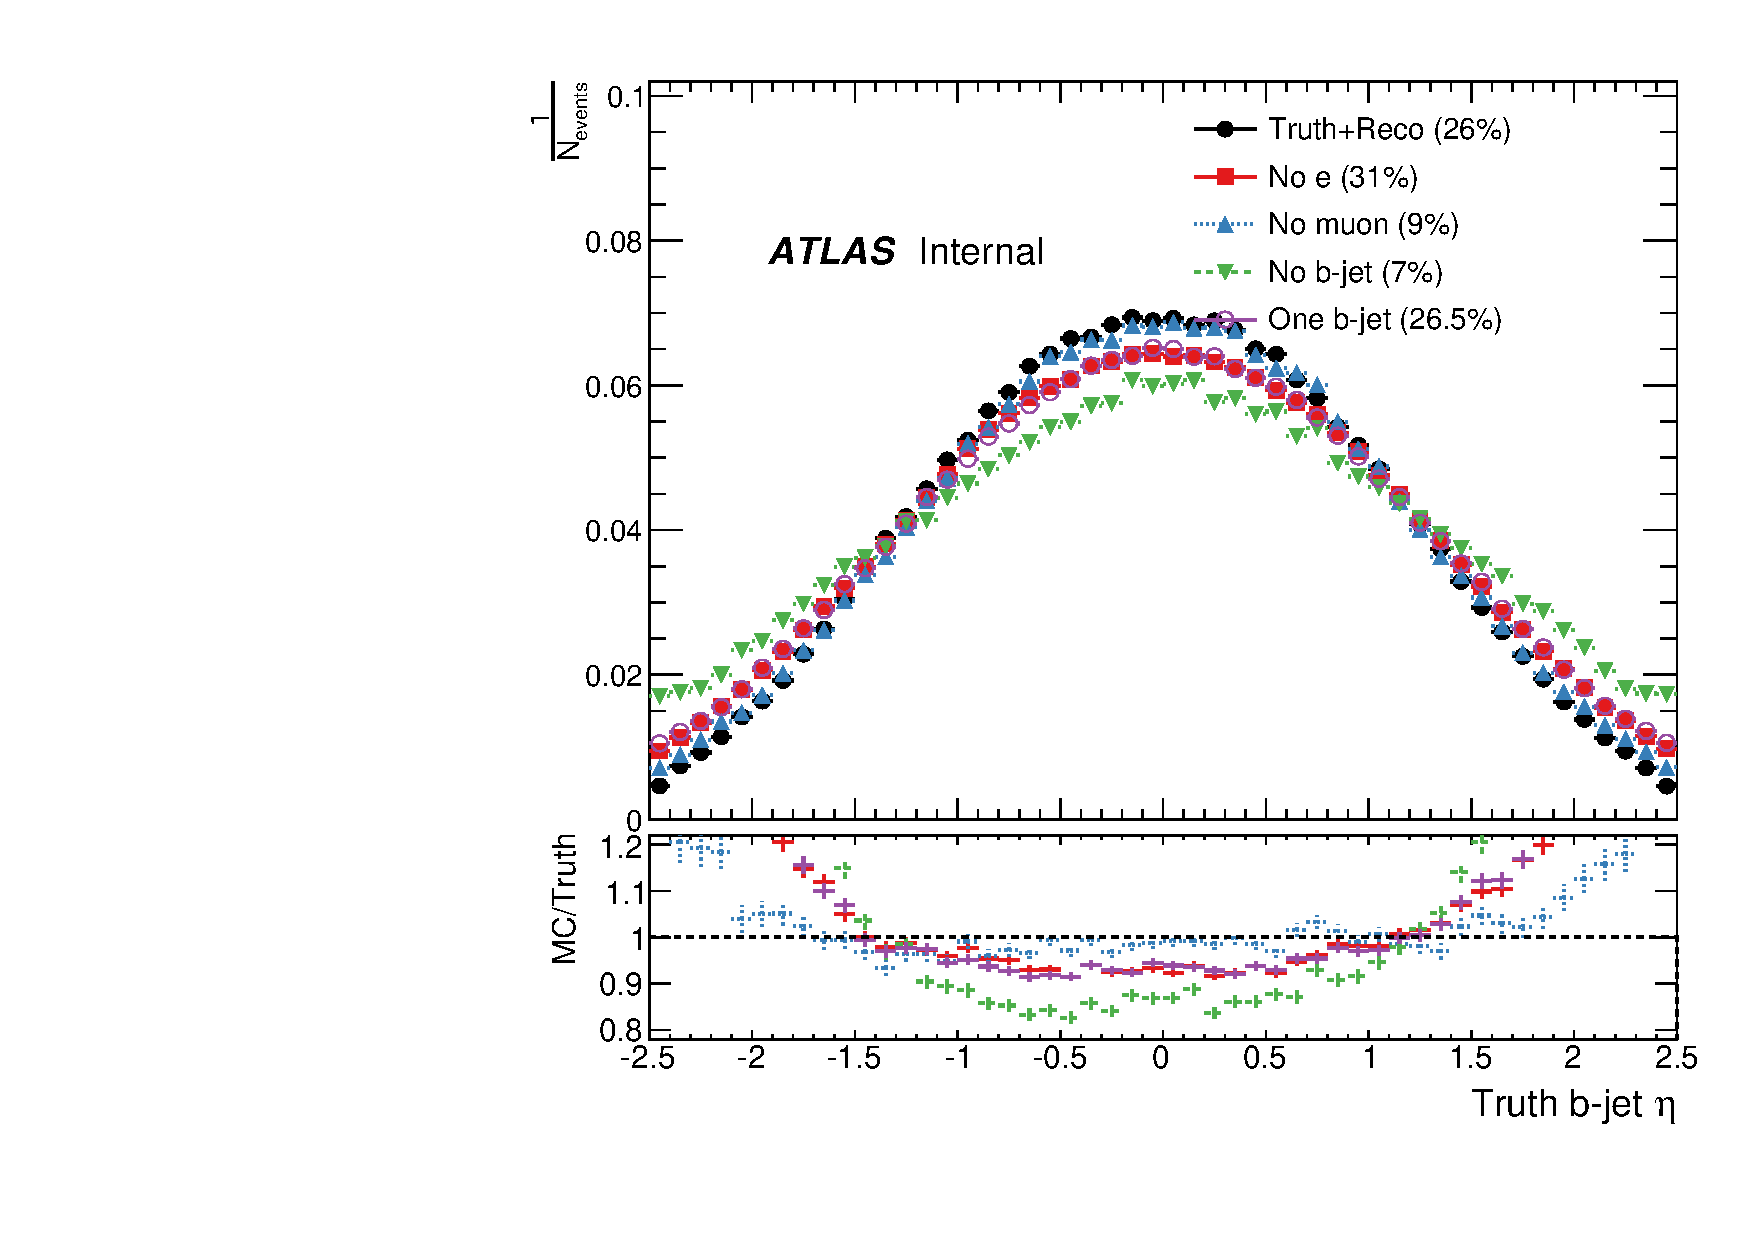
\includegraphics[width=\textwidth]{fig/TruthNotReco/TruthBJetEta.pdf}
\end{subfigure}
\caption{Distributions of the true $b$-jet \pt and $\eta$ for events in different reconstructed categories. Each distribution is normalized by the number of events falling in that category. }
\label{fig:norecobjet}
\end{figure}

\begin{figure}
\centering
\begin{subfigure}[]{0.33\textwidth}
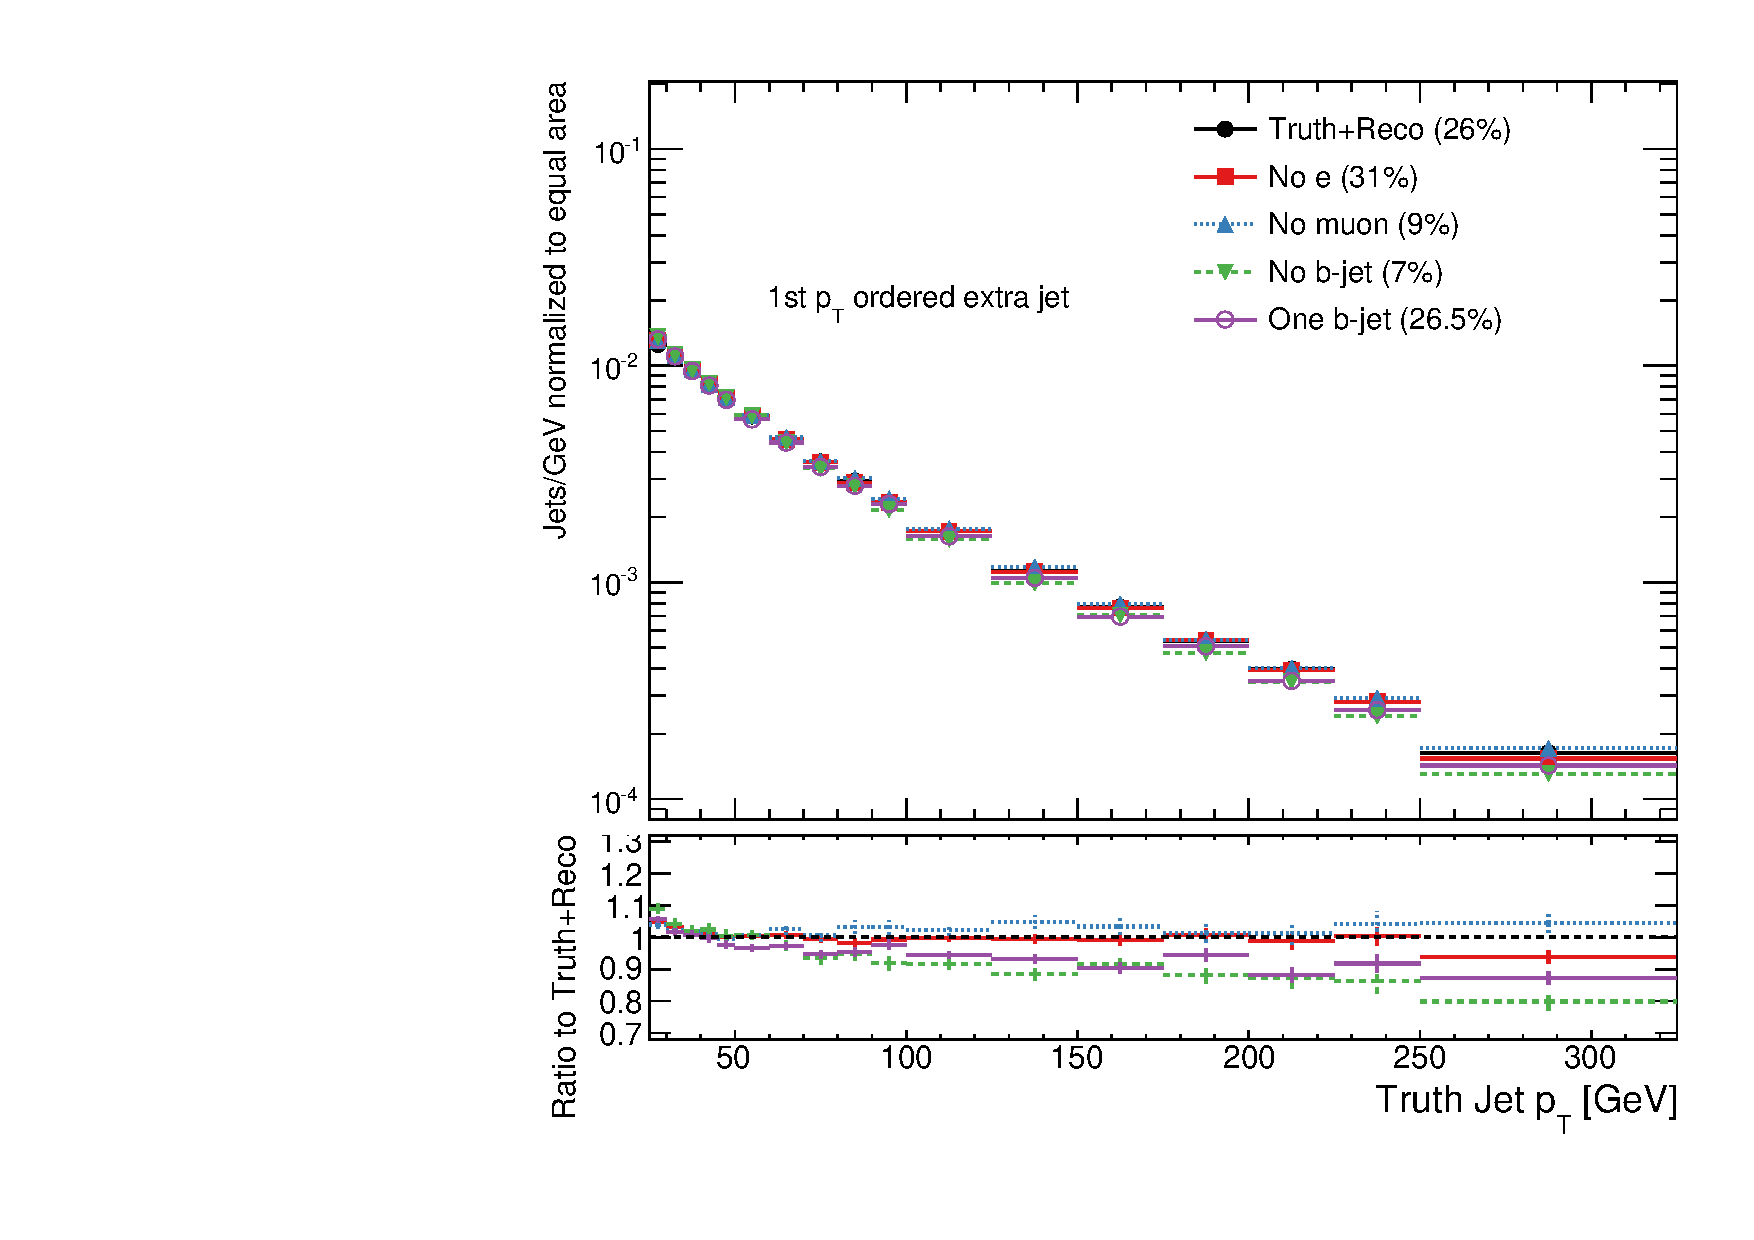
\includegraphics[width=\textwidth]{fig/TruthNotReco/TruthPtJet0.pdf}
\end{subfigure}
~
\begin{subfigure}[]{0.33\textwidth}
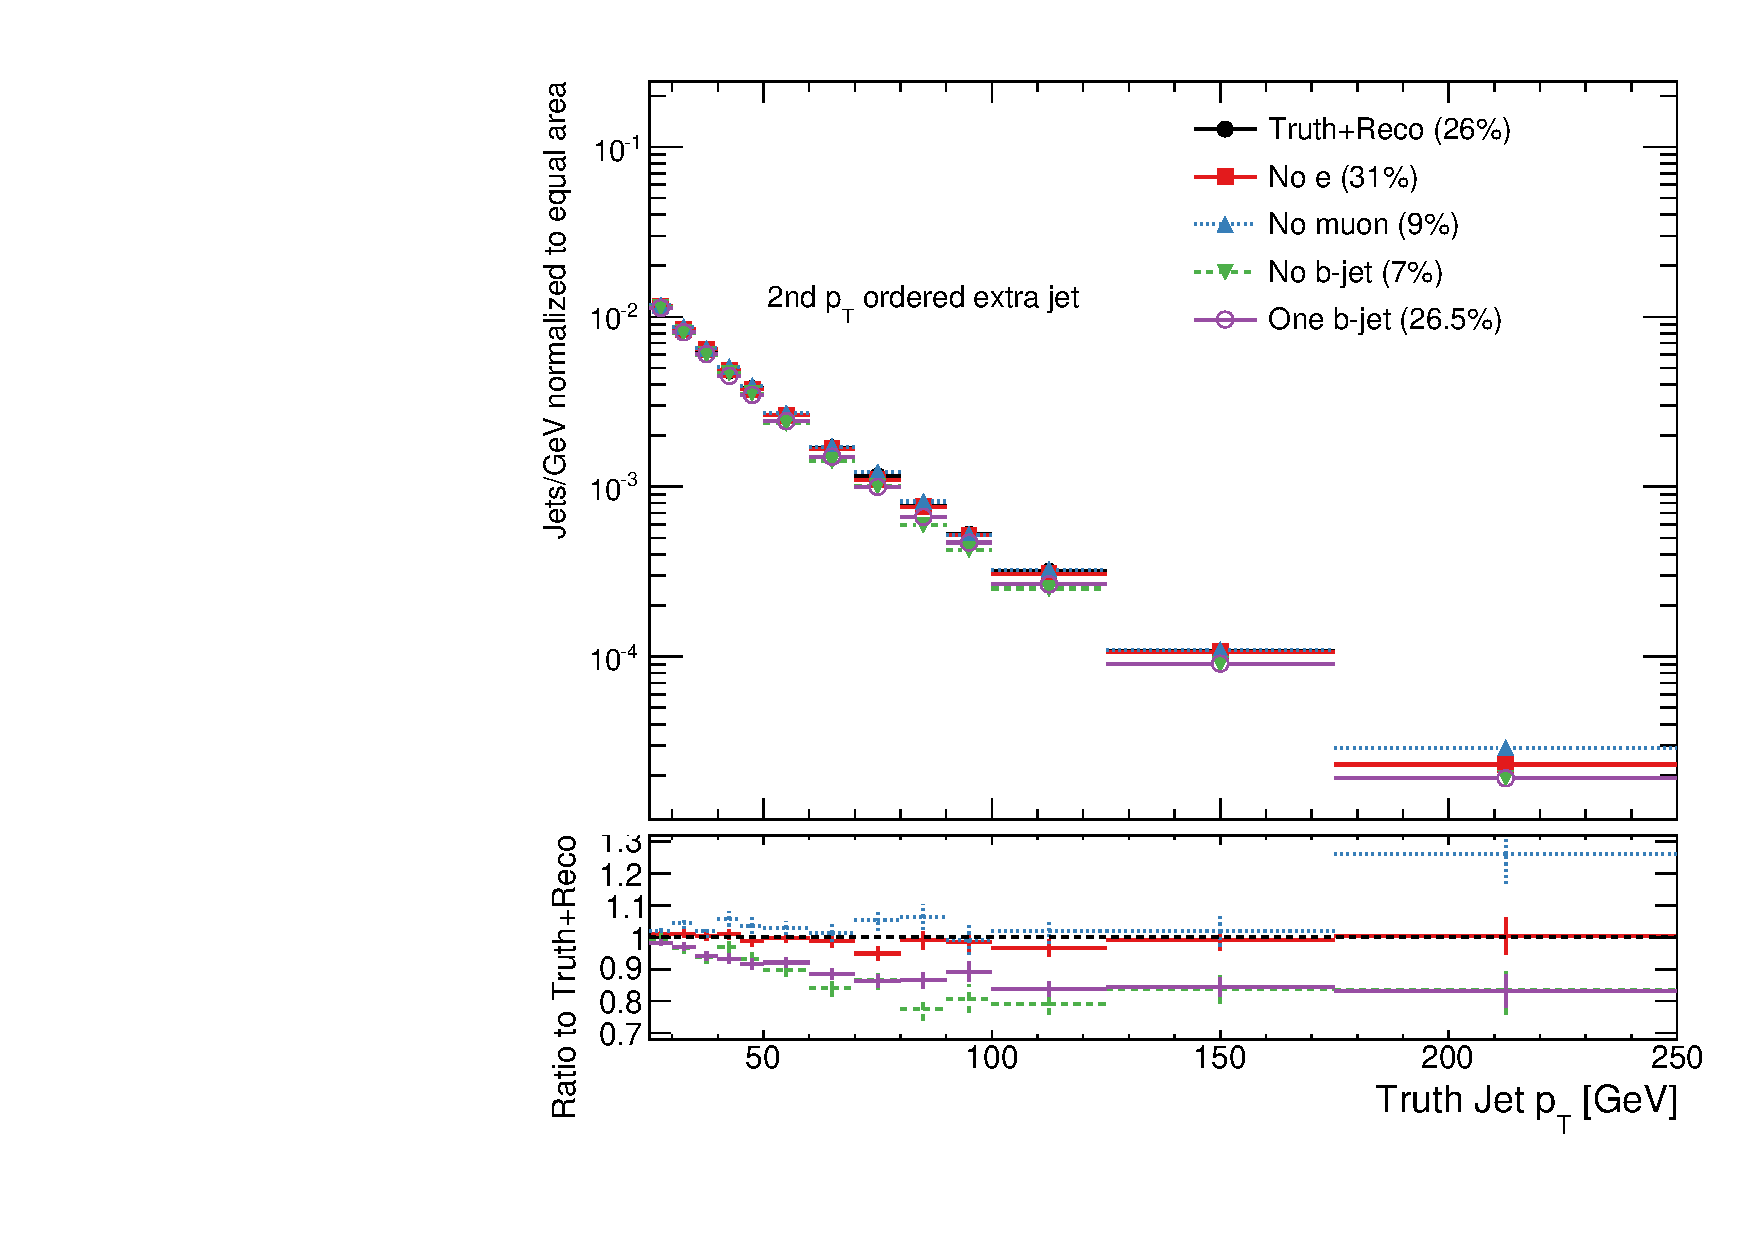
\includegraphics[width=\textwidth]{fig/TruthNotReco/TruthPtJet1.pdf}
\end{subfigure}
\\
\begin{subfigure}[]{0.33\textwidth}
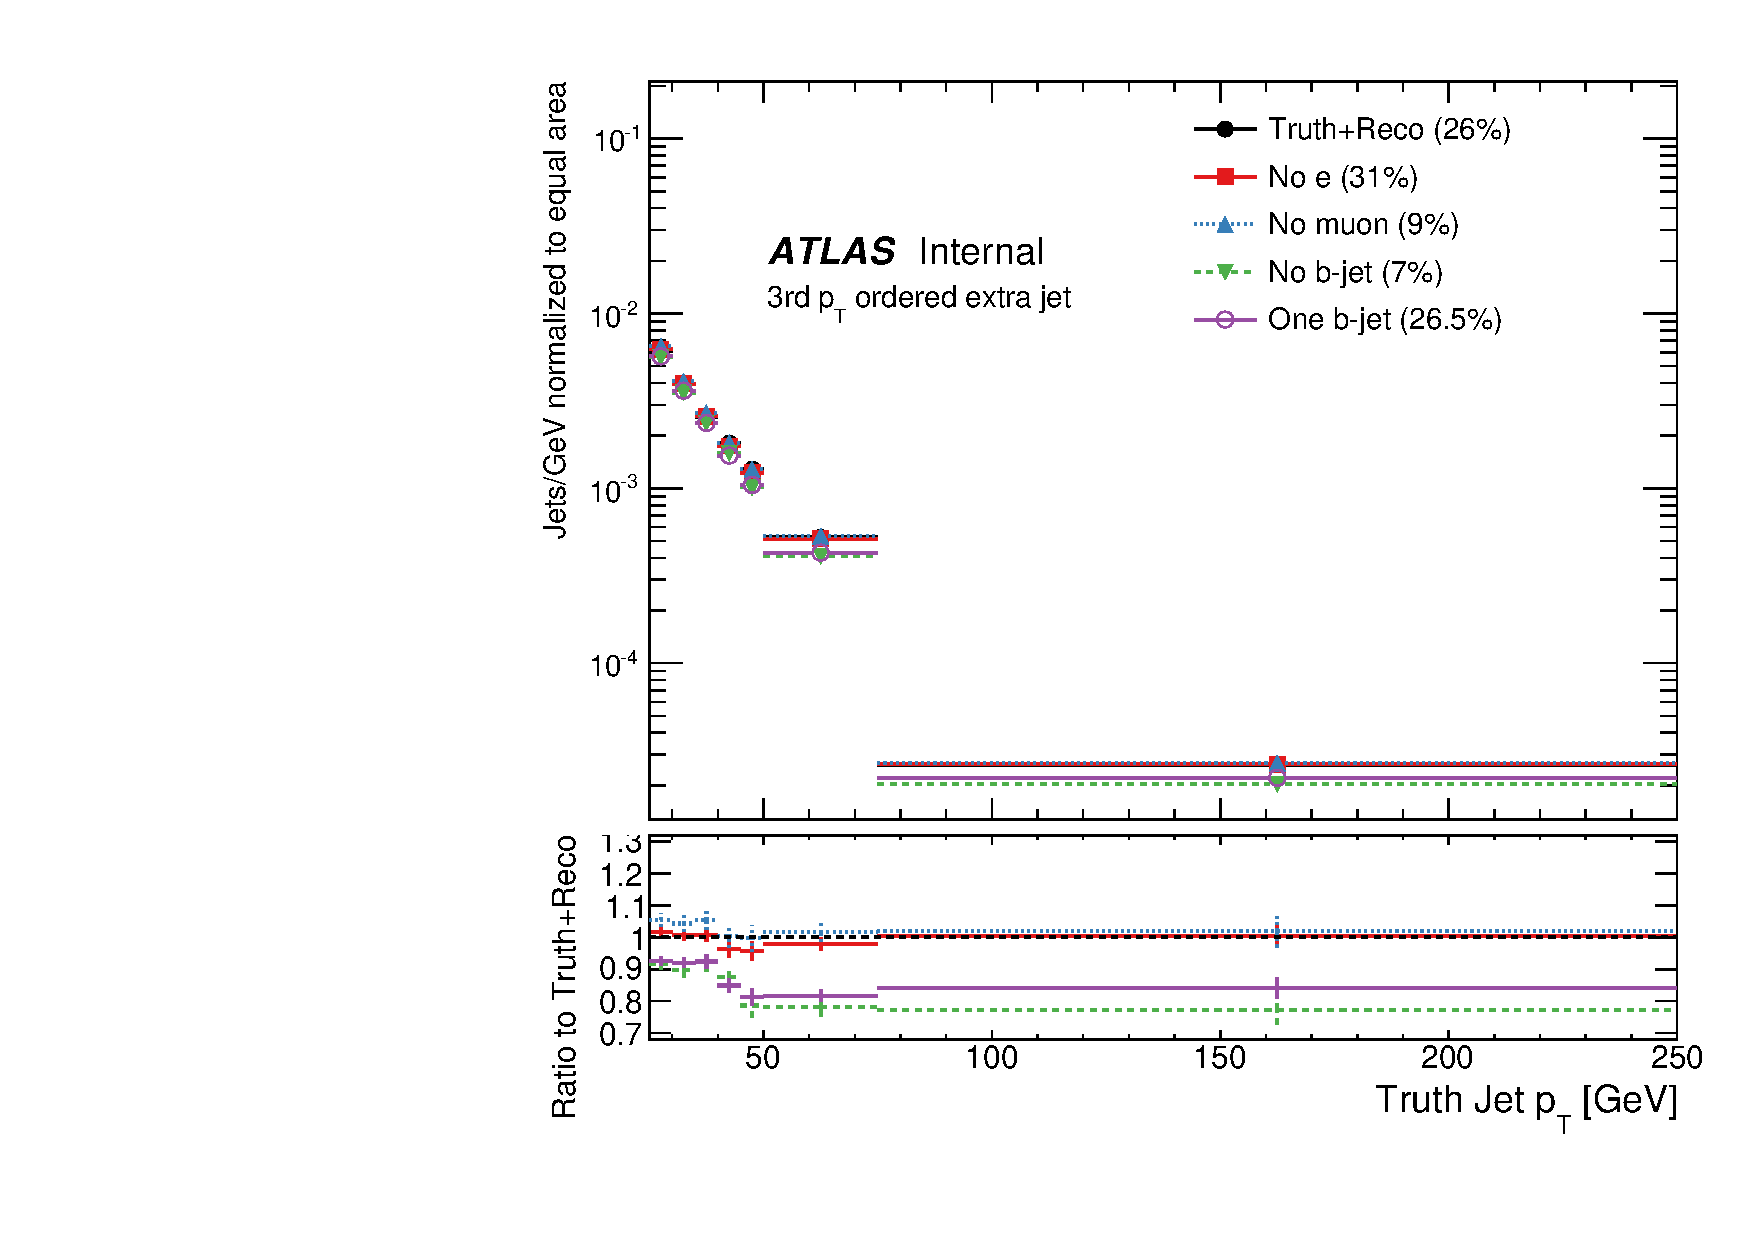
\includegraphics[width=\textwidth]{fig/TruthNotReco/TruthPtJet2.pdf}
\end{subfigure}
~
\begin{subfigure}[]{0.33\textwidth}
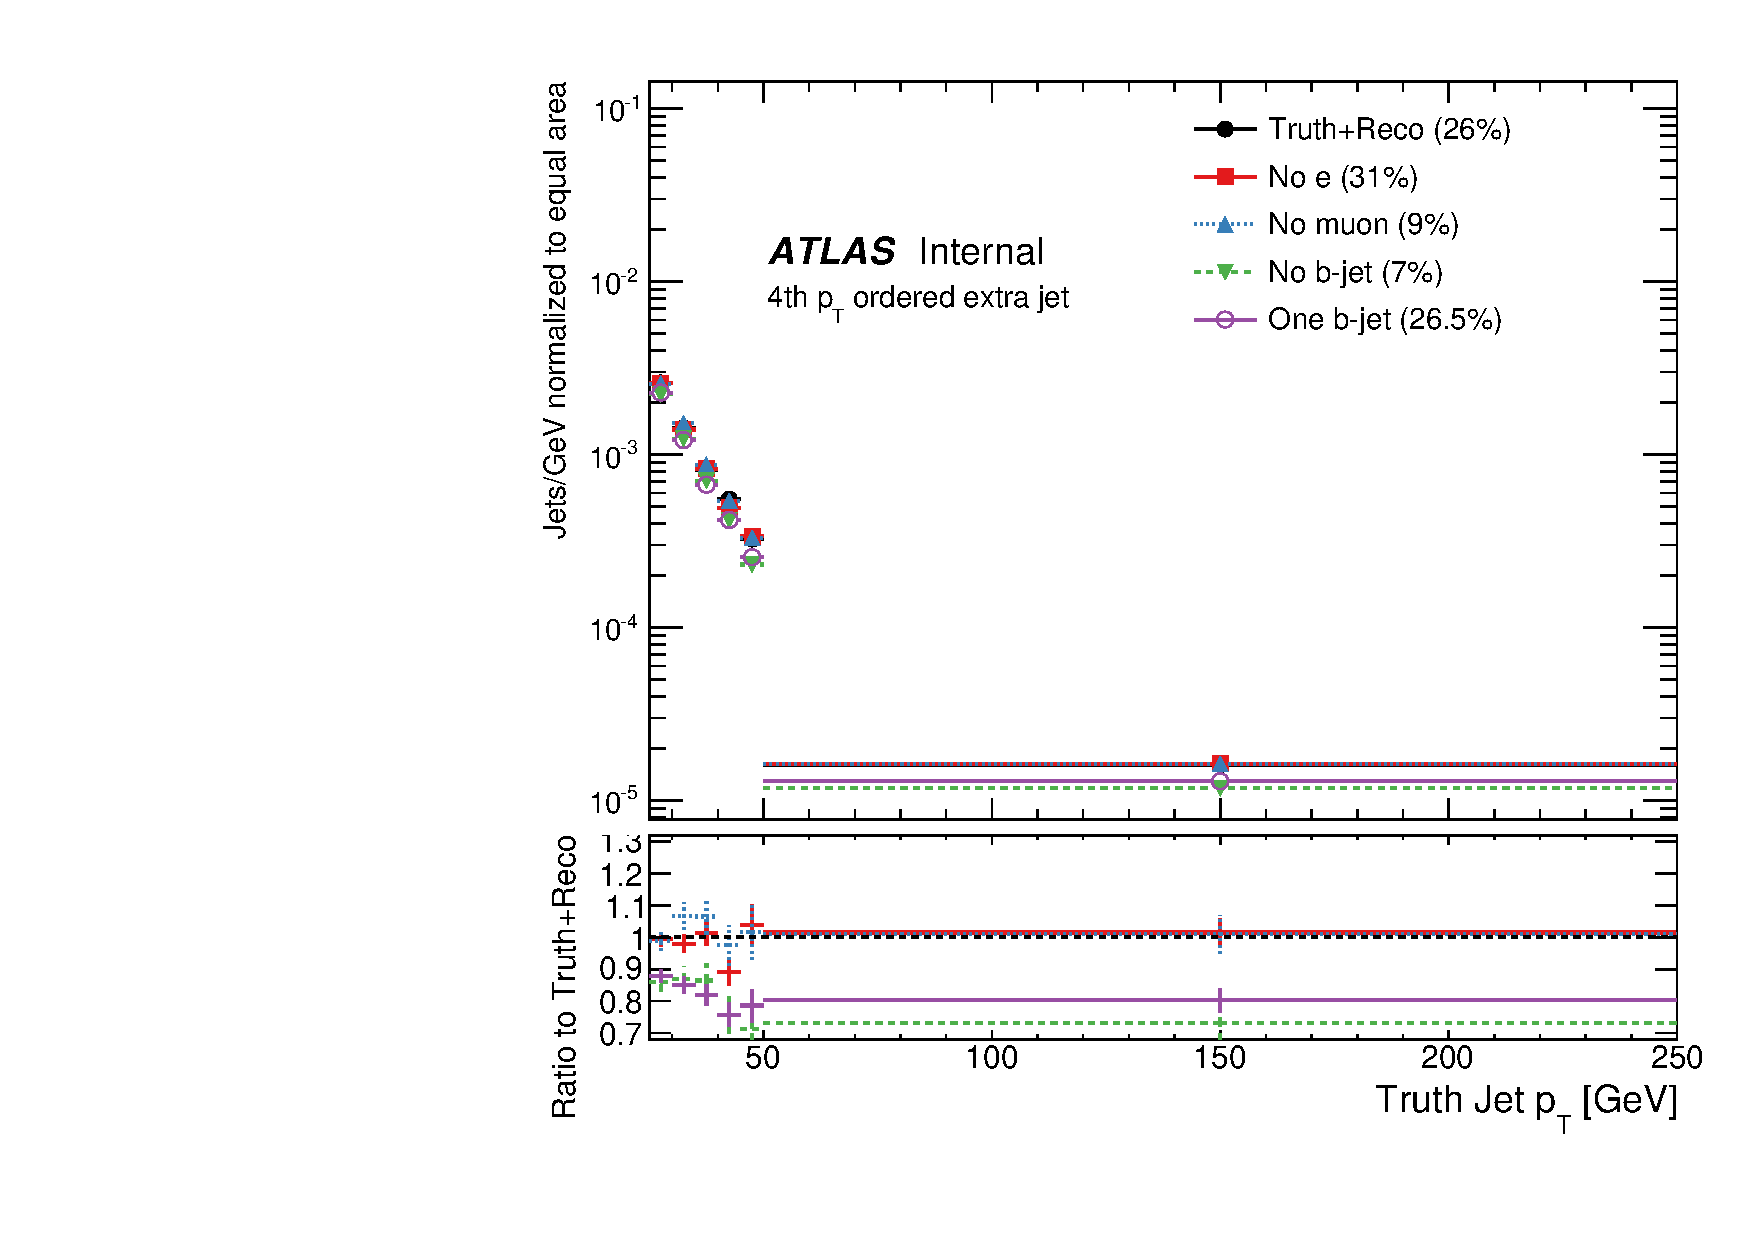
\includegraphics[width=\textwidth]{fig/TruthNotReco/TruthPtJet3.pdf}
\end{subfigure}
~
\\
\begin{subfigure}[]{0.33\textwidth}
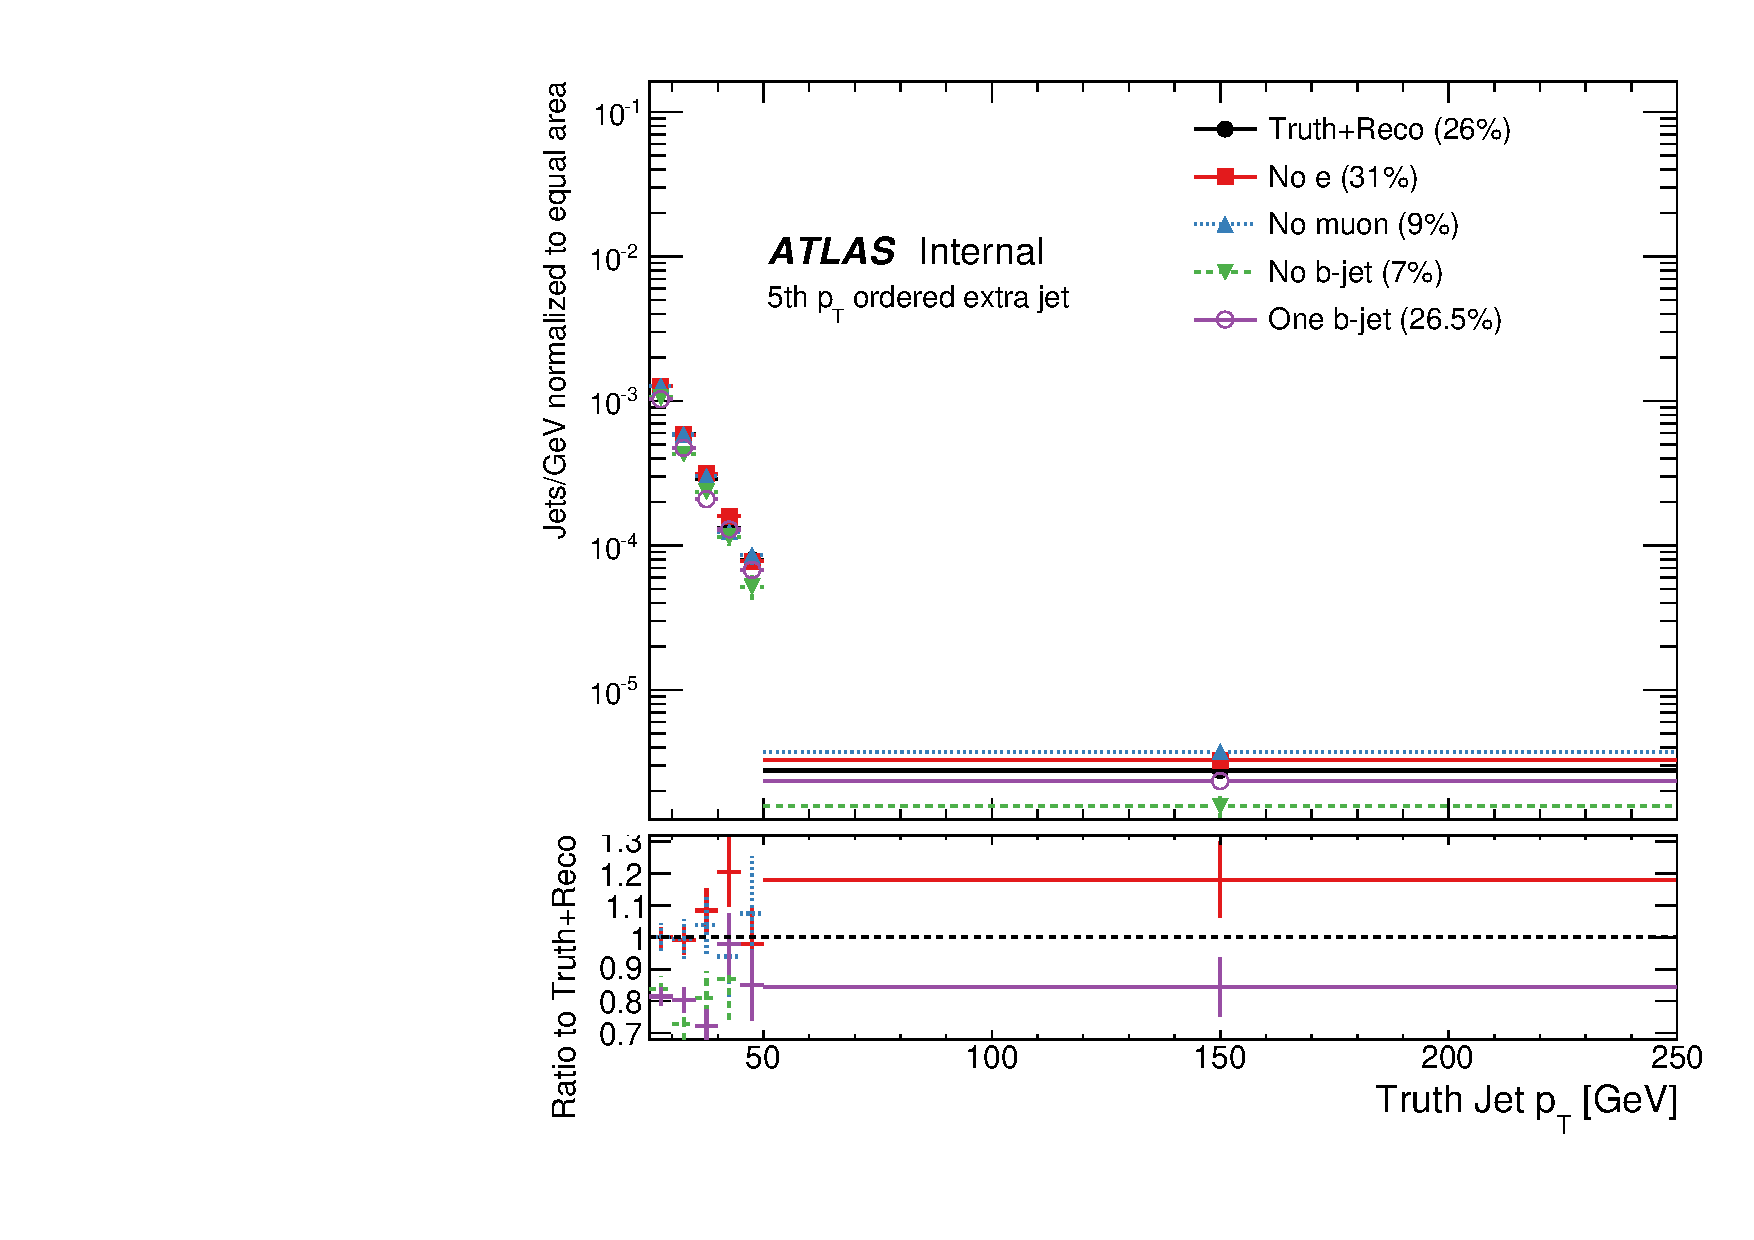
\includegraphics[width=\textwidth]{fig/TruthNotReco/TruthPtJet4.pdf}
\end{subfigure}

\caption{Distributions of the true extra jet extra jet \pt for events in different reconstructed categories. Each distribution is normalized by the number of events falling in that category. }
\label{fig:norecojetpt}
\end{figure}

\begin{figure}
\centering
\begin{subfigure}[]{0.45\textwidth}
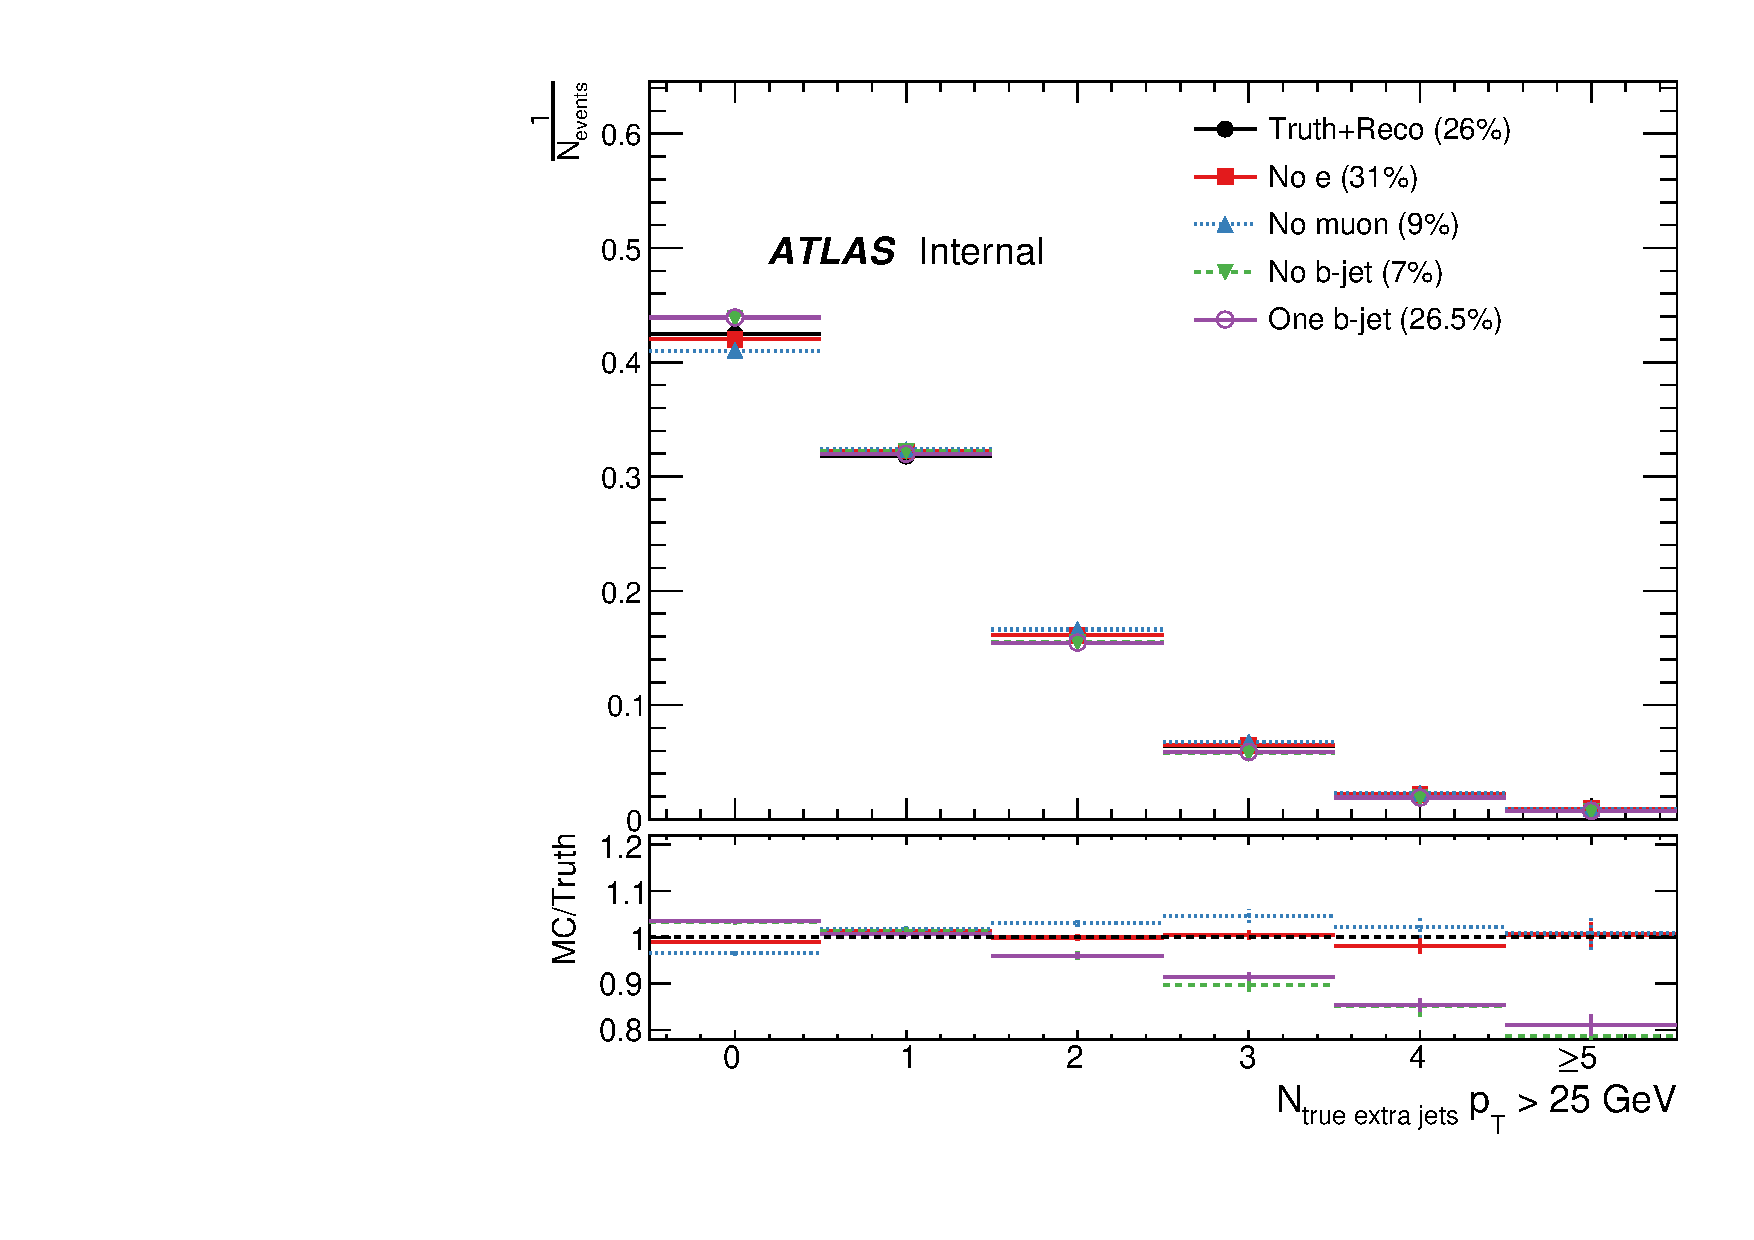
\includegraphics[width=\textwidth]{fig/TruthNotReco/NTruthExtraJets25.pdf}
\end{subfigure}
~
\begin{subfigure}[]{0.45\textwidth}
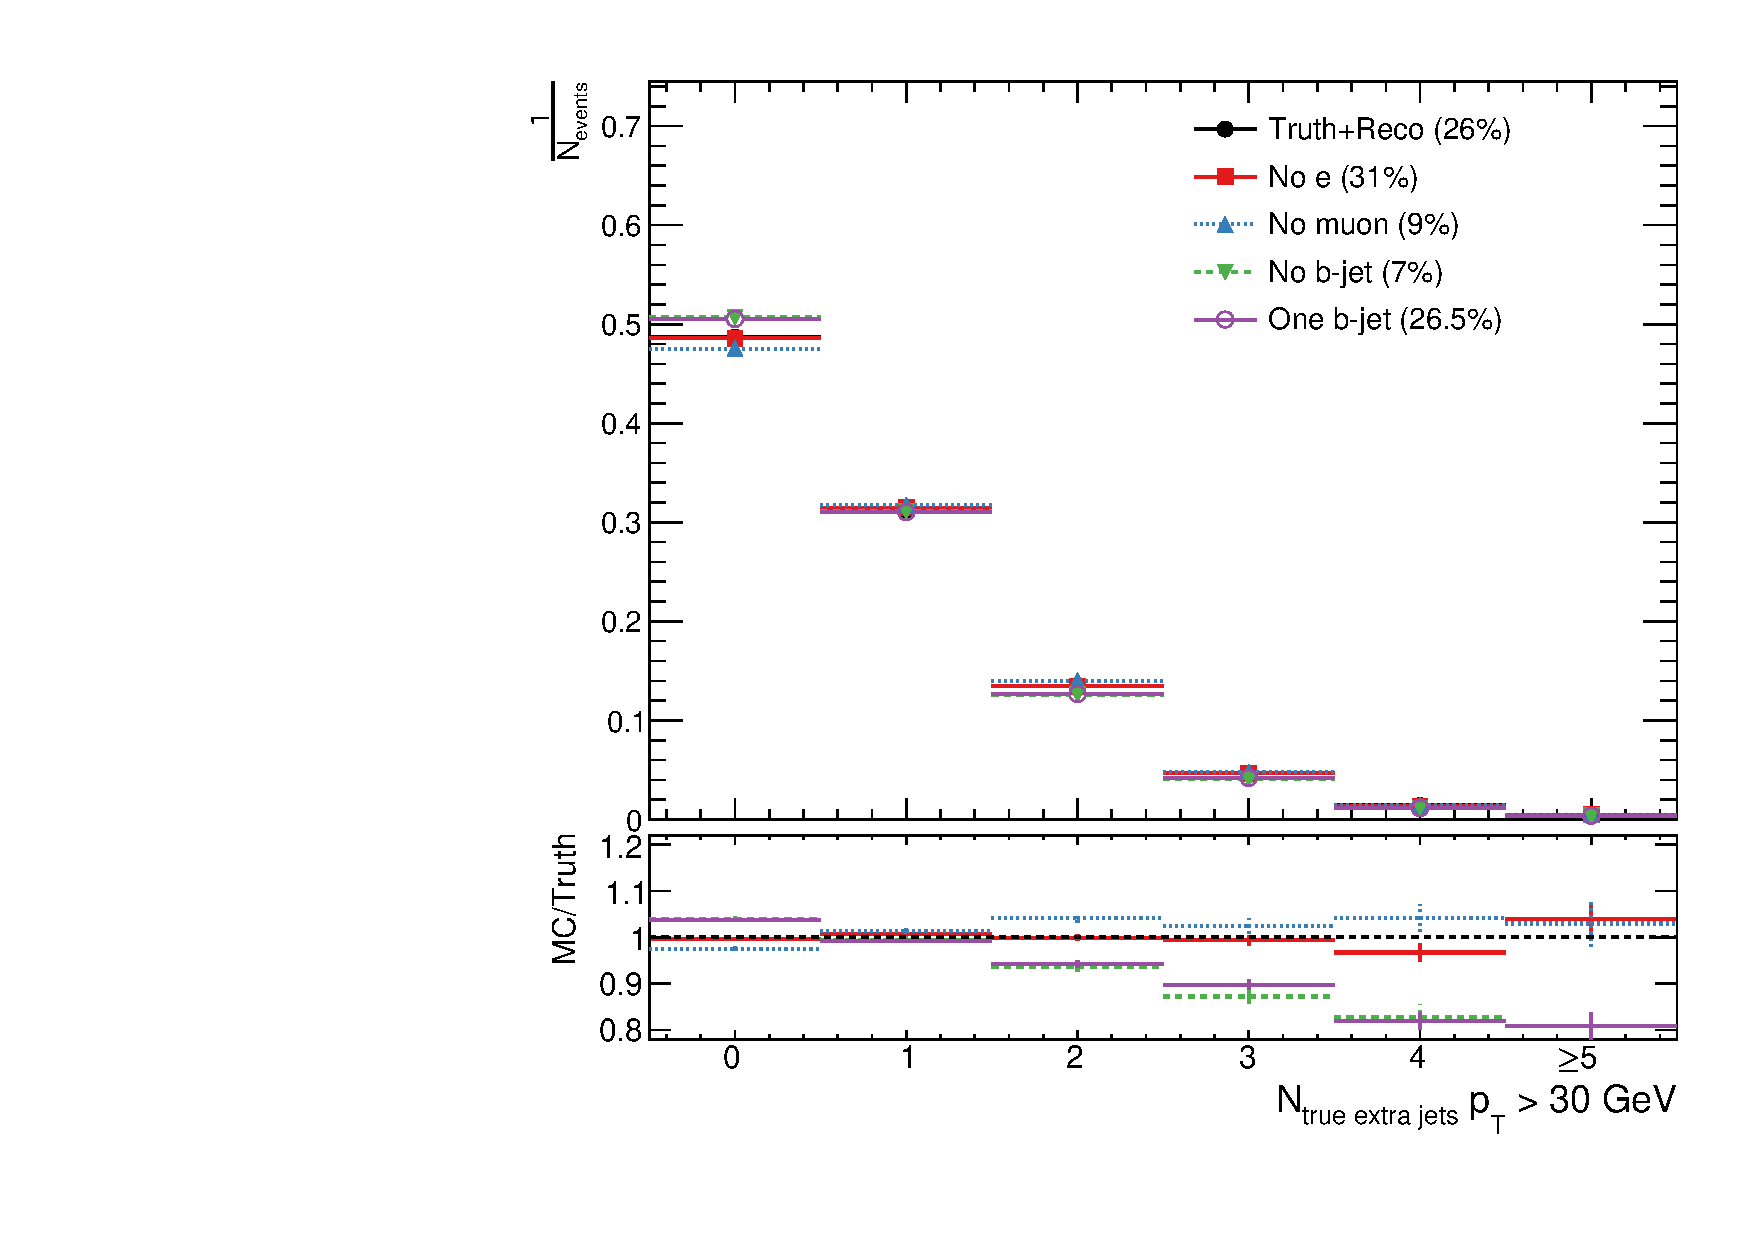
\includegraphics[width=\textwidth]{fig/TruthNotReco/NTruthExtraJets30.pdf}
\end{subfigure}
~
\begin{subfigure}[]{0.45\textwidth}
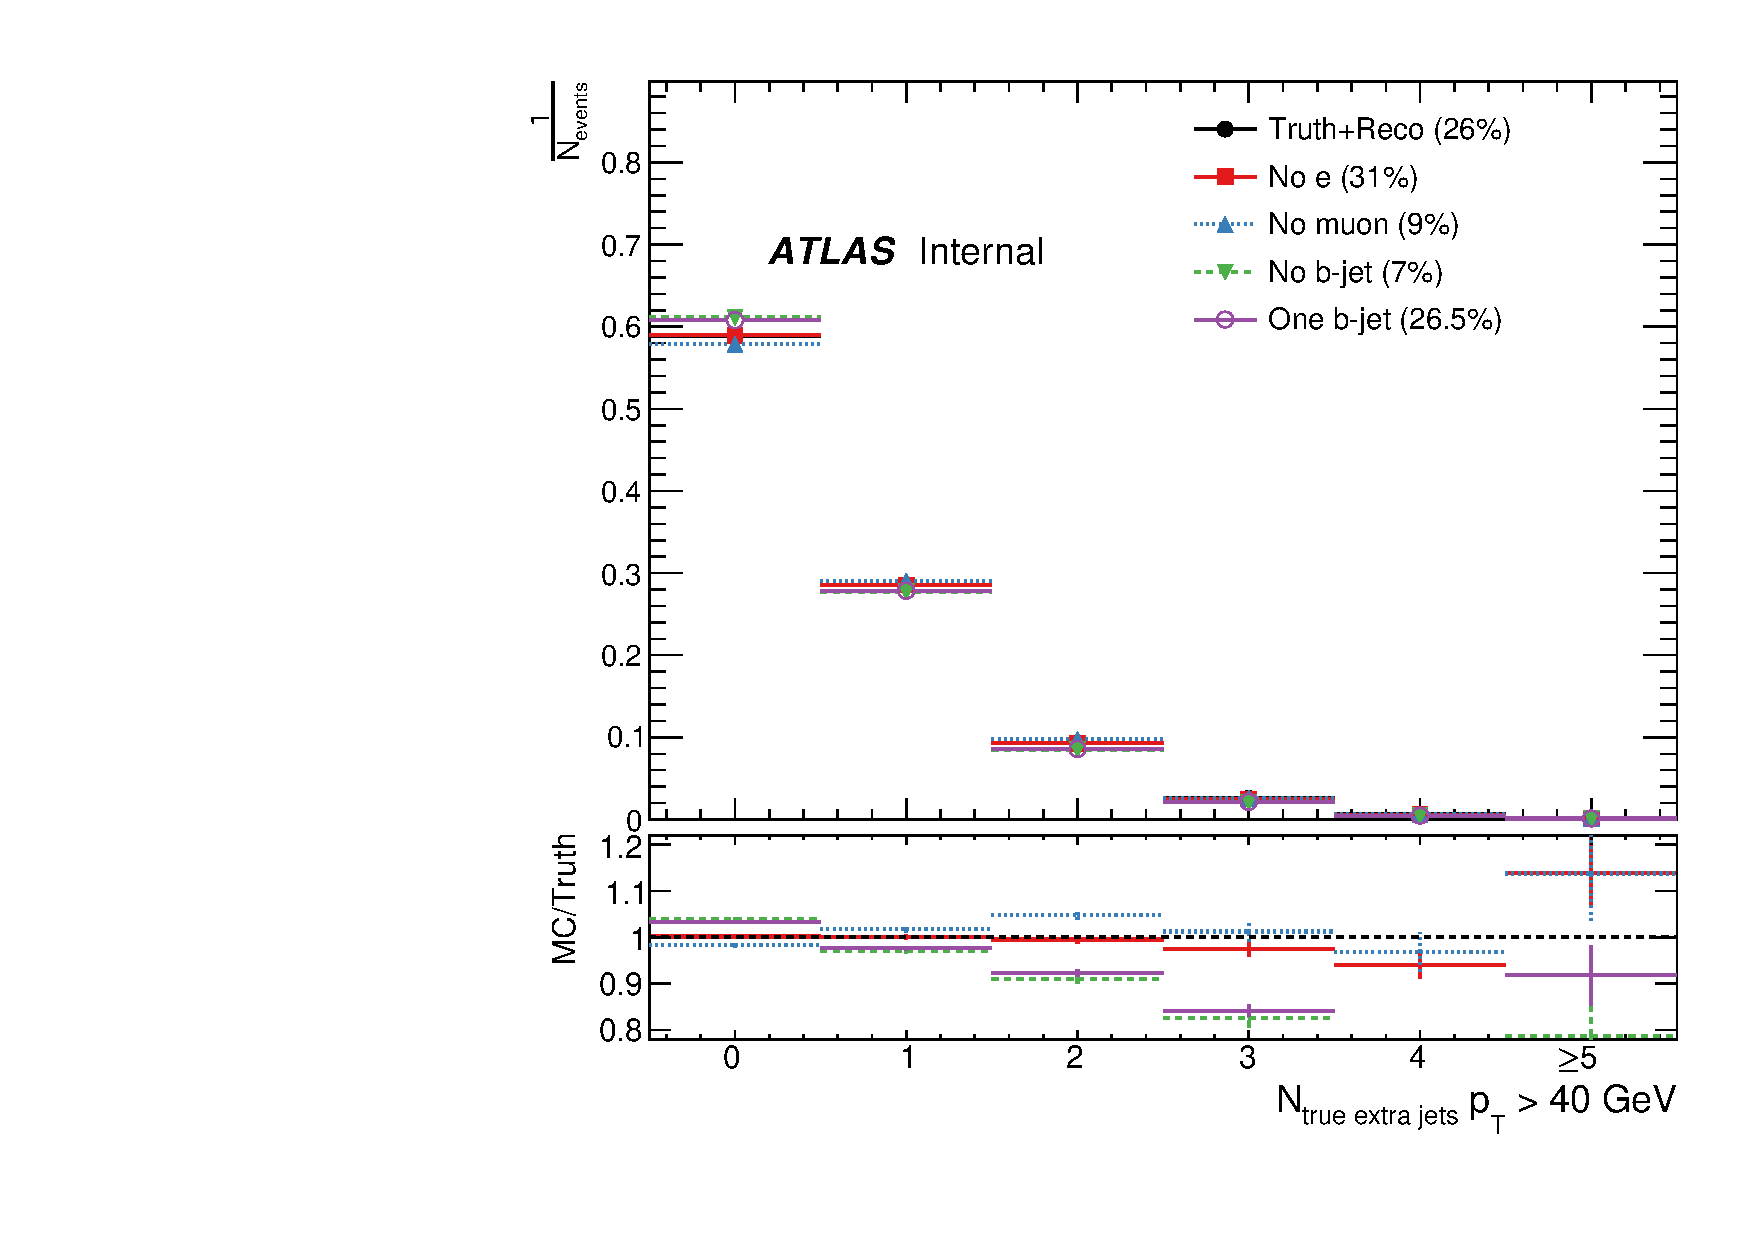
\includegraphics[width=\textwidth]{fig/TruthNotReco/NTruthExtraJets40.pdf}
\end{subfigure}
~
\begin{subfigure}[]{0.45\textwidth}
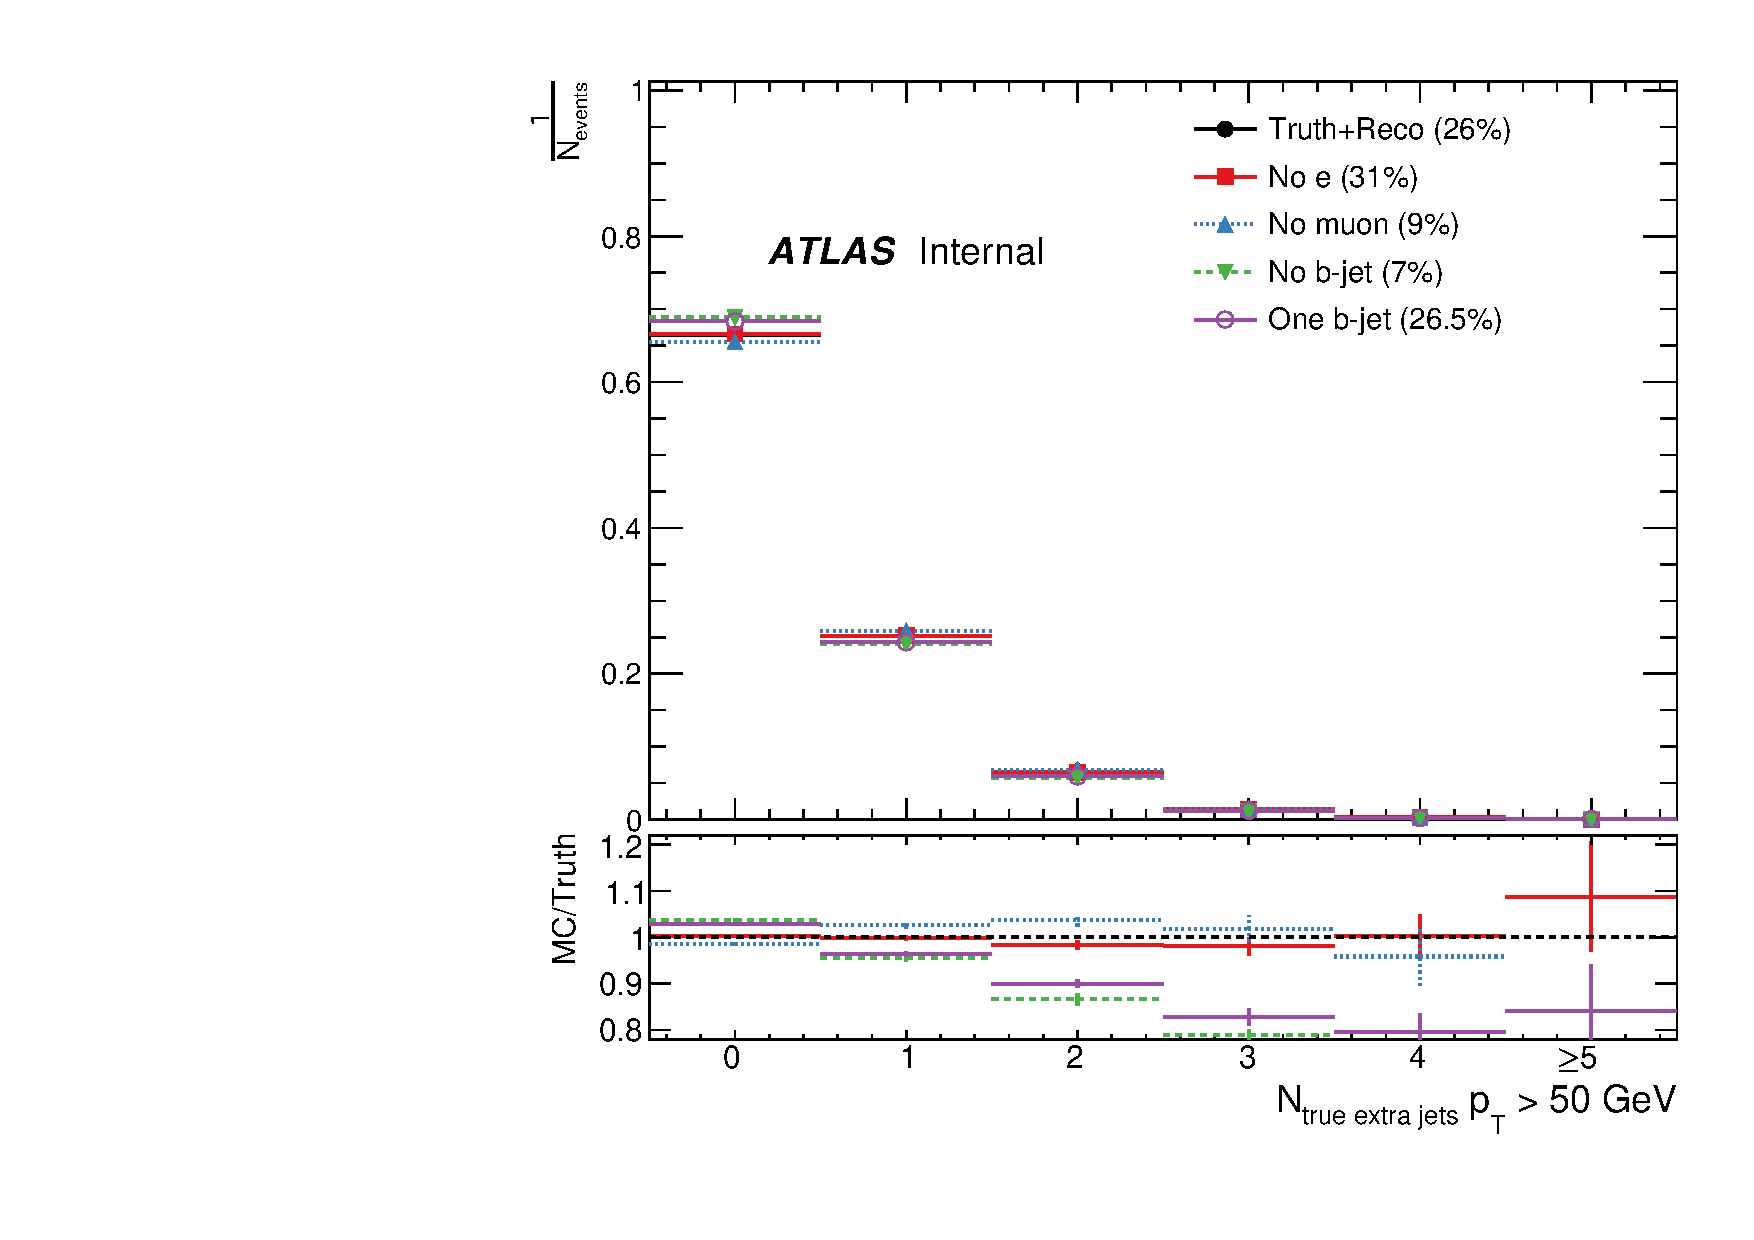
\includegraphics[width=\textwidth]{fig/TruthNotReco/NTruthExtraJets50.pdf}
\end{subfigure}

\caption{Distributions of the true extra jet multiplicity for events in different reconstructed categories. Each distribution is normalized by the number of events falling in that category.}
\label{fig:norecojetmult}

\end{figure}
\clearpage
